\documentclass{article}

\usepackage{graphicx}
\usepackage{tikz}
\usepackage{tikzsymbols}
\usetikzlibrary{calc,patterns,shapes.geometric}
\pagestyle{empty}
\usepackage[margin=0pt]{geometry}
\geometry{papersize={14in,12in}}

\def\centerarc[#1](#2)(#3:#4:#5){\draw[#1] ($(#2)+({#5*cos(#3)},{#5*sin(#3)})$) arc (#3:#4:#5);}

\begin{document}
	\begin{figure}
		\centering
		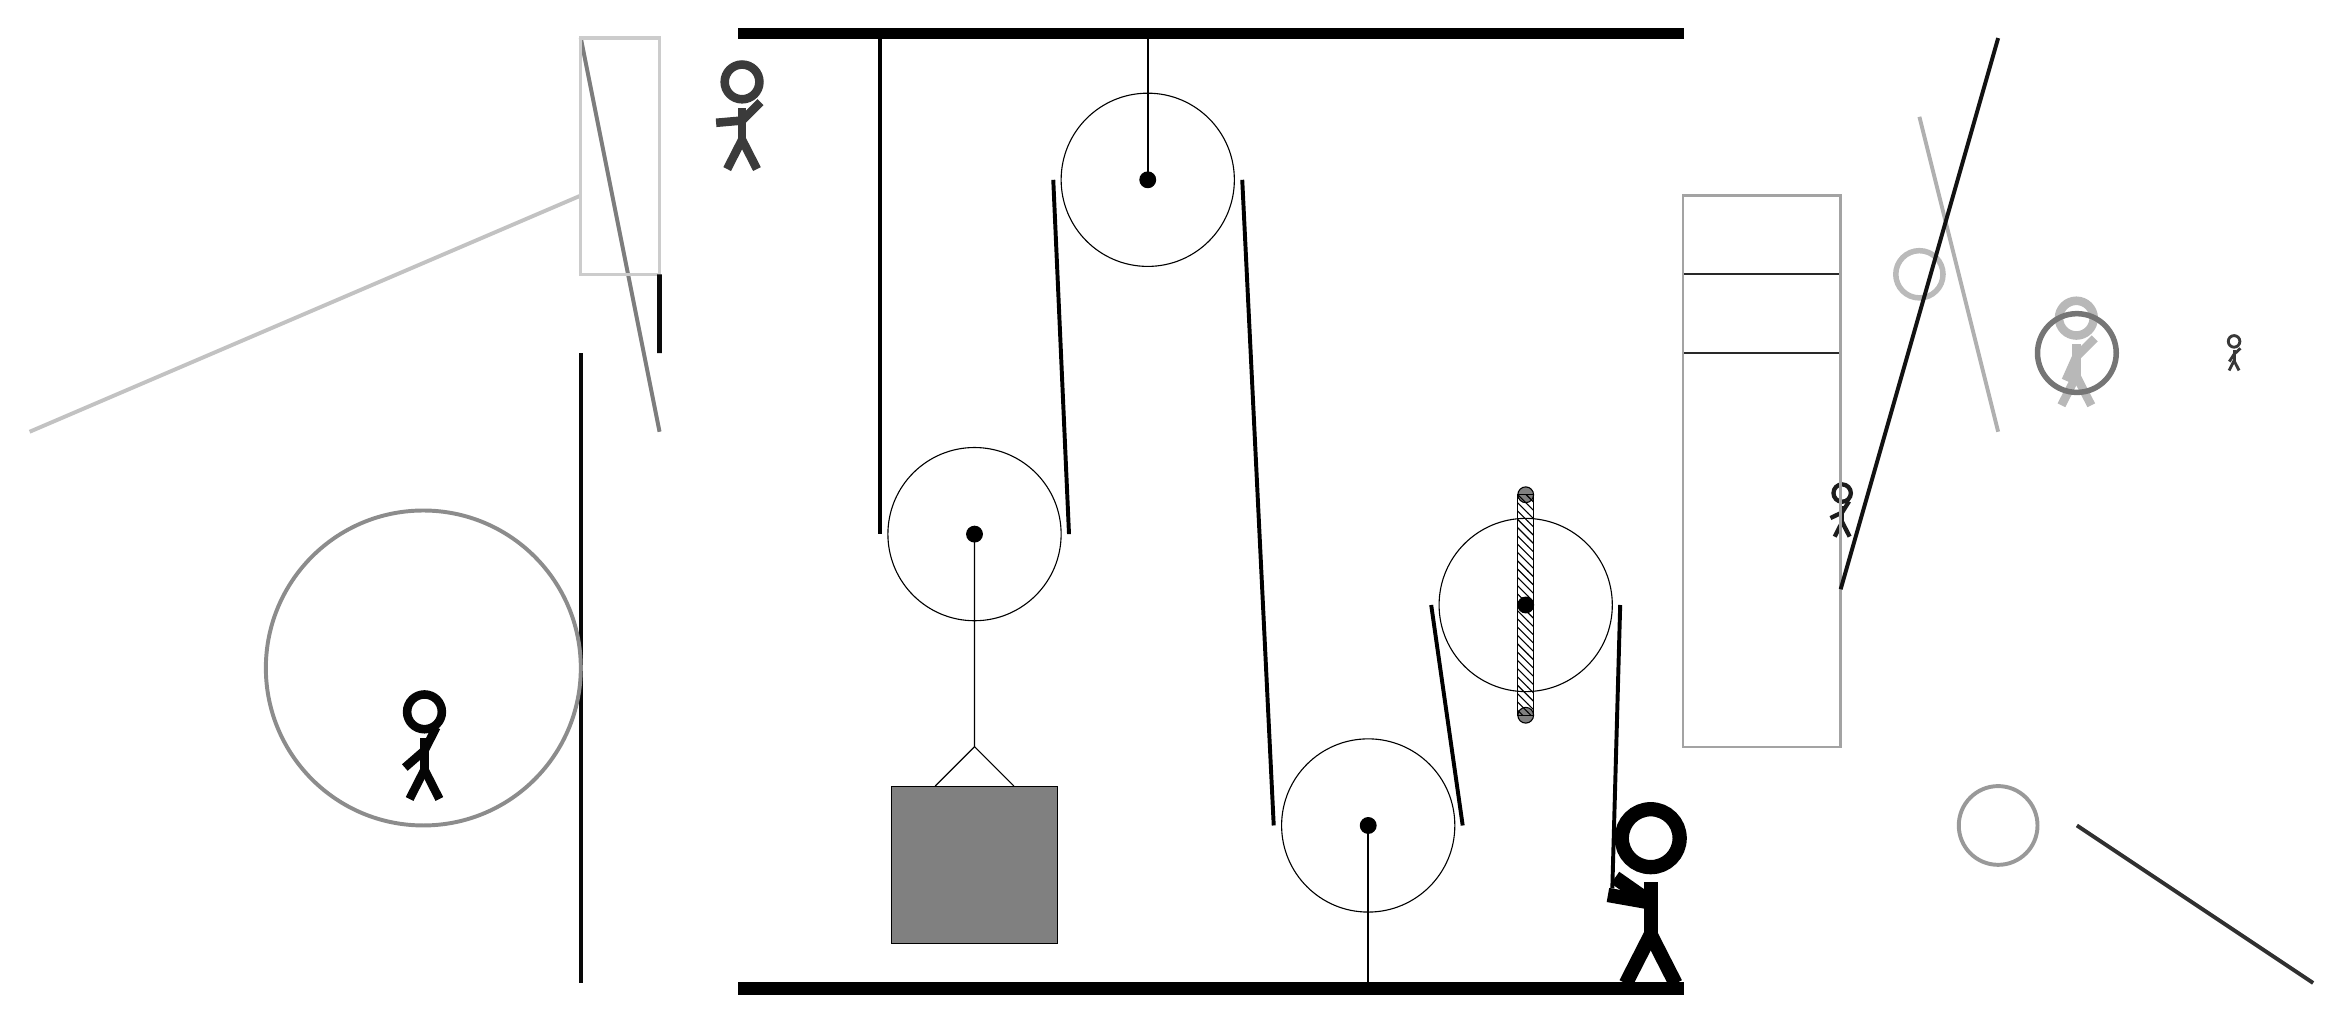
\begin{tikzpicture}
			%%%%% START %%%%%
			
			\draw[fill=black] (-2, 9) rectangle (10, 9.125);
			
			\draw (1, 2.7) circle (1.1);
			\draw[fill=black] (1, 2.7) circle (0.1);
			
			\draw (3.2, 7.2) circle (1.1);
			\draw[fill=black] (3.2, 7.2) circle (0.1);
			\draw[thick] (3.2, 7.2) -- (3.2, 9);
			
			\draw (6, -1) circle (1.1);
			\draw[fill=black] (6, -1) circle (0.1);
			\draw[thick] (6, -1) -- (6, -3);
			
			\draw[fill=white](8, 1.8) circle (1.1);
			\draw[fill=black] (8, 1.8) circle (0.1);
			\draw[fill=black!50] (8, 3.2) circle (0.1);
			\draw[fill=black!50] (8, 0.4) circle (0.1);
			\draw[pattern=north west lines, pattern color=black] (7.9, 3.2) rectangle (8.1, 0.4);
			
			\draw[line width=0.5mm, color=black!51](-4, 9) -- (-3, 4);
			
			\node[line width=0.7mm, color=black!77] at (-2, 8) {\Strichmaxerl[6][5][45]};
			\draw[line width=0.2mm, color=black!84] (10, 6) rectangle (12, 5);
			\draw[line width=0.5mm, color=black!31](14, 4) -- (13, 8);
			\node[line width=0.4mm, color=black!89] at (12, 3) {\Strichmaxerl[3][26][58]};
			
			\draw [line width=0.7mm, color=black!27](13, 6) circle (0.3);
			\draw[line width=0.3mm, color=black!36] (12, 7) rectangle (10, 0);
			\draw[line width=0.5mm, color=black!24](-4, 7) -- (-11, 4);
			\node[line width=0.5mm, color=black!28] at (15, 5) {\Strichmaxerl[6][66][45]};
			\draw[line width=0.4mm, color=black!20] (-4, 9) rectangle (-3, 6);
			\draw[line width=0.5mm, color=black!97](-4, 5) -- (-4, -3);
			\draw [line width=0.7mm, color=black!54](15, 5) circle (0.5);
			\draw[line width=0.5mm, color=black!93](12, 2) -- (14, 9);
			
			\draw[line width=0.6mm, color=black!96] (-3, 5) rectangle (-3, 6);
			\draw [line width=0.5mm, color=black!45](-6, 1) circle (2.0);
			\draw [line width=0.5mm, color=black!40](14, -1) circle (0.5);
			
			\draw[line width=0.5mm, color=black!81](15, -1) -- (18, -3);
			
			\node[line width=0.5mm, color=black!78] at (17, 5) {\Strichmaxerl[2][57][43]};
			\node[line width=0.4mm, color=black!98] at (-6, 0) {\Strichmaxerl[6][41][63]};
			
			\draw (1, 2.7) -- (1, 0) -- (0.5, -0.5);
			\draw (1, 0) -- (1.5, -0.5);
			\draw[fill=black!50] (-0.05, -0.5) rectangle (2.05, -2.5);
			
			\draw[line width=0.5mm] (-0.2, 9) -- (-0.2, 2.7);
			\centerarc[line width=0.5mm](1, 2.7)(180:360:1.2000000000000002);
			\draw[line width=0.5mm](2.2, 2.7) -- (2.0, 7.2);
			\centerarc[line width=0.5mm](3.2, 7.2)(0:180:1.2000000000000002);
			\draw[line width=0.5mm](4.4, 7.2) -- (4.8, -1);
			\centerarc[line width=0.5mm](6, -1)(180:360:1.2000000000000002);
			\draw[line width=0.5mm](7.2, -1) -- (6.8, 1.8);
			\centerarc[line width=0.5mm](8, 1.8)(0:180:1.2000000000000002);
			\draw[line width=0.5mm](9.2, 1.8) -- (9.1, -1.8);
			
			\node at (9.5, -1.9) {\Strichmaxerl[10][-35][170]};
			
			\draw[fill=black] (-2, -3) rectangle (10, -3.15);
			
			%%%%% END %%%%%
		\end{tikzpicture}
	\end{figure}	
\end{document}